\begin{wrapfigure}{r}{0.45\textwidth}
\centering
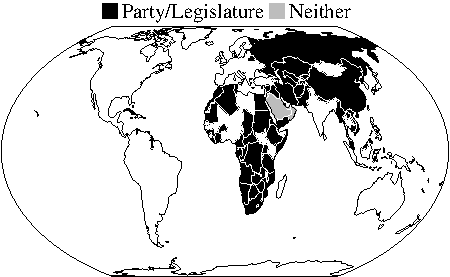
\includegraphics[width=1\linewidth]{./sections/01intro/worldmapTermpaperIntro.pdf}
\caption{Parties and legislatures in authoritarian regimes, 2007}
\label{fig:worldmapIntro}
\end{wrapfigure}
Contemporary research holds that co-optation and political 
repression represent two mainstays of authoritarian regimes 
\citep[21f.]{Gerschewski.2013}. Usually co-optation 
is defined as ``the intentional extension of benefits to 
potential challengers to the regime in exchange for their 
loyalty'' \citep[333]{Frantz.2014}, and legislatures and 
parties are said to simplify those exchanges. Since 
the end of the Cold War those nominally democratic 
institutions have taken root in almost every authoritarian 
regime. In fact, by 2007 only Saudi Arabia, Oman, and the 
United Arab Emirates sustained neither political parties nor
a publicly elected parliament. At the same time, however, 
authoritarian regimes did not forget about political 
repression. Restrictions on core political liberties 
and violations of physical integrity rights limit public 
criticism of the government, they undermine coordinated 
campaigns against it, and occasionally they even enforce 
commitments in authoritarian politics 
\citep[33,38]{Wintrobe.1998}. Yet, little is know about how 
co-optation and political repression interact.

This is the point of departure for Erica Frantz' and Andrea 
Kendall-Taylor's \citeyearpar{Frantz.2014} recent publication 
`A dictator’s toolkit: Understanding how co-optation affects 
repression in autocracies'. Based on extensive quantitative 
analyses they claim that co-optation has far-reaching 
consequences for how repression is used 
\citep[332]{Frantz.2014}. More precisely, they find that 
increasing levels of co-optation lead dictators to reduce 
restrictions on empowerment rights, but at the same time 
they increase physical integrity violations. The authors 
explain this key finding by reference to the trade-offs 
involved in applying political repression. Restrictions on 
empowerment such as the freedoms of speech and assembly aim 
at the general public and characterize a diffuse approach to
social control. Physical integrity violations such as 
torture and extra-judicial killings in contrast target 
specific individuals and are more attractive when the 
opposition is known. Nominally democratic institutions offer
fora where regime opponents can make their demands heard and
consequently they increase the available information on the 
political opposition. Under the bottom line, the 
institutions of co-optation generate knowledge on threats to
the regime and lead dictators to ``shift their repressive 
approach in favor of physical integrity rights violations 
over empowerment rights restrictions'' 
\citep[337]{Frantz.2014}.

This paper replicates the work of Frantz and Kendall-Taylor.
It provides evidence to the violation of key assumptions in 
the original publication and raises concerns with regard to
predictive accuracy. Moreover, it casts doubt on a 
widespread estimation strategy that depends on lagged 
dependent variables to control for serial autocorrelation in
pooled time-series cross-sectional designs. My extension \dots.
The following section characterizes data and design of the 
original publication, and section three presents the 
replication results. Section four discusses the results of a
modified estimation approach, and section five concludes.